\documentclass[14pt]{article}
\usepackage{xltxtra}
\usepackage{fontspec}
\usepackage{polyglossia}
\usepackage[margin=1in]{geometry}
\usepackage{booktabs}
\usepackage{graphicx}
\usepackage{tabularx}
\usepackage{ragged2e}
\usepackage{titlesec}
\usepackage{float}

\newcommand{\sectionbreak}{\clearpage}
% Font setup
\setmainfont{Times New Roman}
\setsansfont{Arial}
\setmonofont{Courier New}

% Language setup
\setdefaultlanguage{english}

% Section formatting
\titleformat{\section}{\large\bfseries\sffamily}{\thesection}{1em}{}
\titleformat{\subsection}{\normalsize\bfseries\sffamily}{\thesubsection}{1em}{}

% Header
\usepackage{fancyhdr}
\pagestyle{fancy}
\fancyhf{}
\rhead{Bassel Alshayeb | SPbU 2025}
\lhead{Distributed Miminet Optimization}
\cfoot{\thepage}

\begin{document}

% Title Page
\begin{titlepage}
    \centering
    \vspace*{1cm}
    \vspace{1cm}
    {\LARGE\sffamily\bfseries Optimization of Distributed Network Simulation in Miminet Using Docker\par}
    \vspace{2cm}
    \vspace{1cm}
    {\large\sffamily Bassel Alshayeb\par}
    {\large\sffamily Saint Petersburg State University\par}
    {\large\sffamily Faculty of Mathematics and Mechanics\par}

    \vfill
    {\large\sffamily 2025\par}
\end{titlepage}

% Introduction
\section{Introduction}
Computer Networks education is essential for Software Engineering students at SPbU's Faculty of Mathematics and Mechanics. Understanding network principles not only strengthens their knowledge but prepares them for work in systems administration, cybersecurity, and cloud computing.

Traditionally, the practical parts of the course involved expensive hardware like Cisco\cite{cisco} switches, routers, and complex topologies. However, after Cisco's\cite{cisco} market exit in 2022, acquiring this hardware became financially and logistically impractical.

As a solution, Miminet\cite{miminet}, a lightweight network emulator based on Mininet\cite{mininet} and Docker, was introduced. Miminet\cite{miminet} offers an affordable and scalable way to emulate computer networks without expensive physical devices. Yet, it suffers from resource bottlenecks due to its single-container architecture, especially when many students perform simulations concurrently.

\textbf{Objective:} This project focuses on optimizing Miminet's\cite{miminet} simulation execution by distributing the workload across multiple Docker containers, significantly improving performance and scalability.

% Related Work
\section{Related Work}
Mininet\cite{mininet} has been widely used for network simulation, however, it typically operates within a single namespace, limiting scalability. Some modern approaches in network research apply container-based deployments (e.g., Kubernetes network testing), but require heavy resource overheads.

Miminet\cite{miminet} seeks to balance lightweight operation with scalability. Therefore, enhancing Miminet\cite{miminet} to support distributed execution is a practical step toward making it a real educational and experimental platform.

% Implementation
\section{Implementation}
\subsection{Architecture Overview}
The system redesign splits Miminet\cite{miminet} instances across several containers, each handling a subset of network simulations. Task distribution is managed through a distributed queue.

\subsection{Problem Statement}

Miminet\cite{miminet} uses a centralized simulation management model, where:
\begin{itemize}
    \item The entire simulation is executed inside a single Docker container.
    \item Virtual nodes and connections are created using Linux network namespaces and emulated Ethernet interfaces.
    \item The simulation is controlled via the Mininet\cite{mininet} Python\cite{python} API, providing for the configuration of nodes, switches, and routers.
    \item The entire process is executed in a single environment, which limits scalability as the number of nodes increases.
\end{itemize}

\begin{figure}[h!]
    \centering
    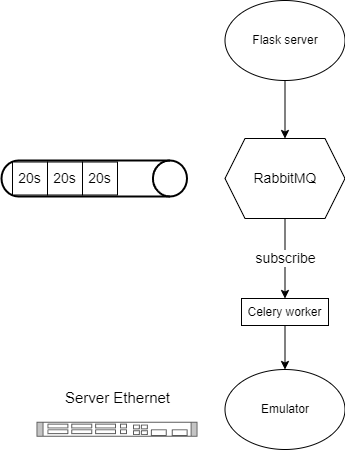
\includegraphics[width=0.4\textwidth]{seq.png}
    \caption{Current Single-Container Miminet Architecture}
\end{figure}

Miminet's\cite{miminet} single-container model causes:
\begin{itemize}
    \item High simulation latency under load
    \item Underutilization of available CPU cores
    \item Sequential task execution without concurrency
\end{itemize}
These factors limited the scalability and usability of the emulator.

\section{Proposed Solution}
An optimized distributed system was developed using:
\begin{itemize}
    \item Multiple Docker containers for concurrent simulation
    \item Celery\cite{celery} for task distribution
    \item RabbitMQ\cite{rabbitmq} as the messaging broker
\end{itemize}
Simulation requests are dynamically scheduled to available containers.

\begin{figure}[h!]
    \centering
    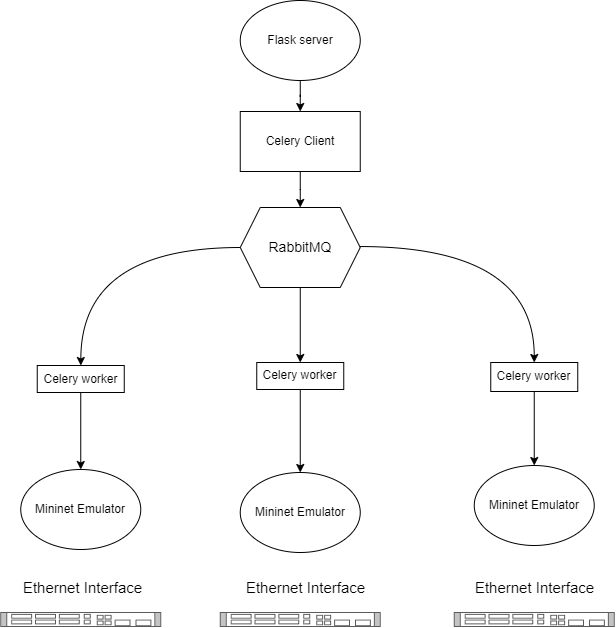
\includegraphics[width=0.4\textwidth]{example.png}
    \caption{Optimized Distributed Miminet Architecture}
\end{figure}

\vspace{10pt}
\noindent\textbf{System Components:}
\begin{tabularx}{\linewidth}{lX}
    \toprule
    Component & Functionality \\ \midrule
    Docker Containers & Host isolated Miminet\cite{miminet} instances \newline  \newline
    Celery\cite{celery} Workers & Execute network simulations \newline \newline
    RabbitMQ\cite{rabbitmq} & Message queue broker \newline \newline
    Flask API & Web interface for user interaction \newline \newline
    SQLite DB & Store task metadata and results \\ \bottomrule
\end{tabularx}

\subsection{Workflow}
\begin{enumerate}
    \item Student submits network topology via Flask API.
    \item Task is queued in RabbitMQ\cite{rabbitmq}.
    \item Celery\cite{celery} workers pick up available tasks and start simulations.
    \item Results are collected and returned to the student.
\end{enumerate}


% Results
\section{Performance Results}
Experimental testing shows significant improvement:
\begin{table}[h]
    \centering
    \begin{tabular}{lcc}
        \toprule
        Metric & Single-Container & Distributed \\ \midrule
        Avg. Simulation Time & 10 sec & 4 sec \\
        Max Parallel Simulations & 1 & 10+ \\
        CPU Utilization & 10\% & 80\% \\
        Student Wait Time & 300 sec & 120 sec \\
        \bottomrule
    \end{tabular}
    \caption{Performance Comparison Between Architectures}
\end{table}

\begin{figure}[h!]
\centering
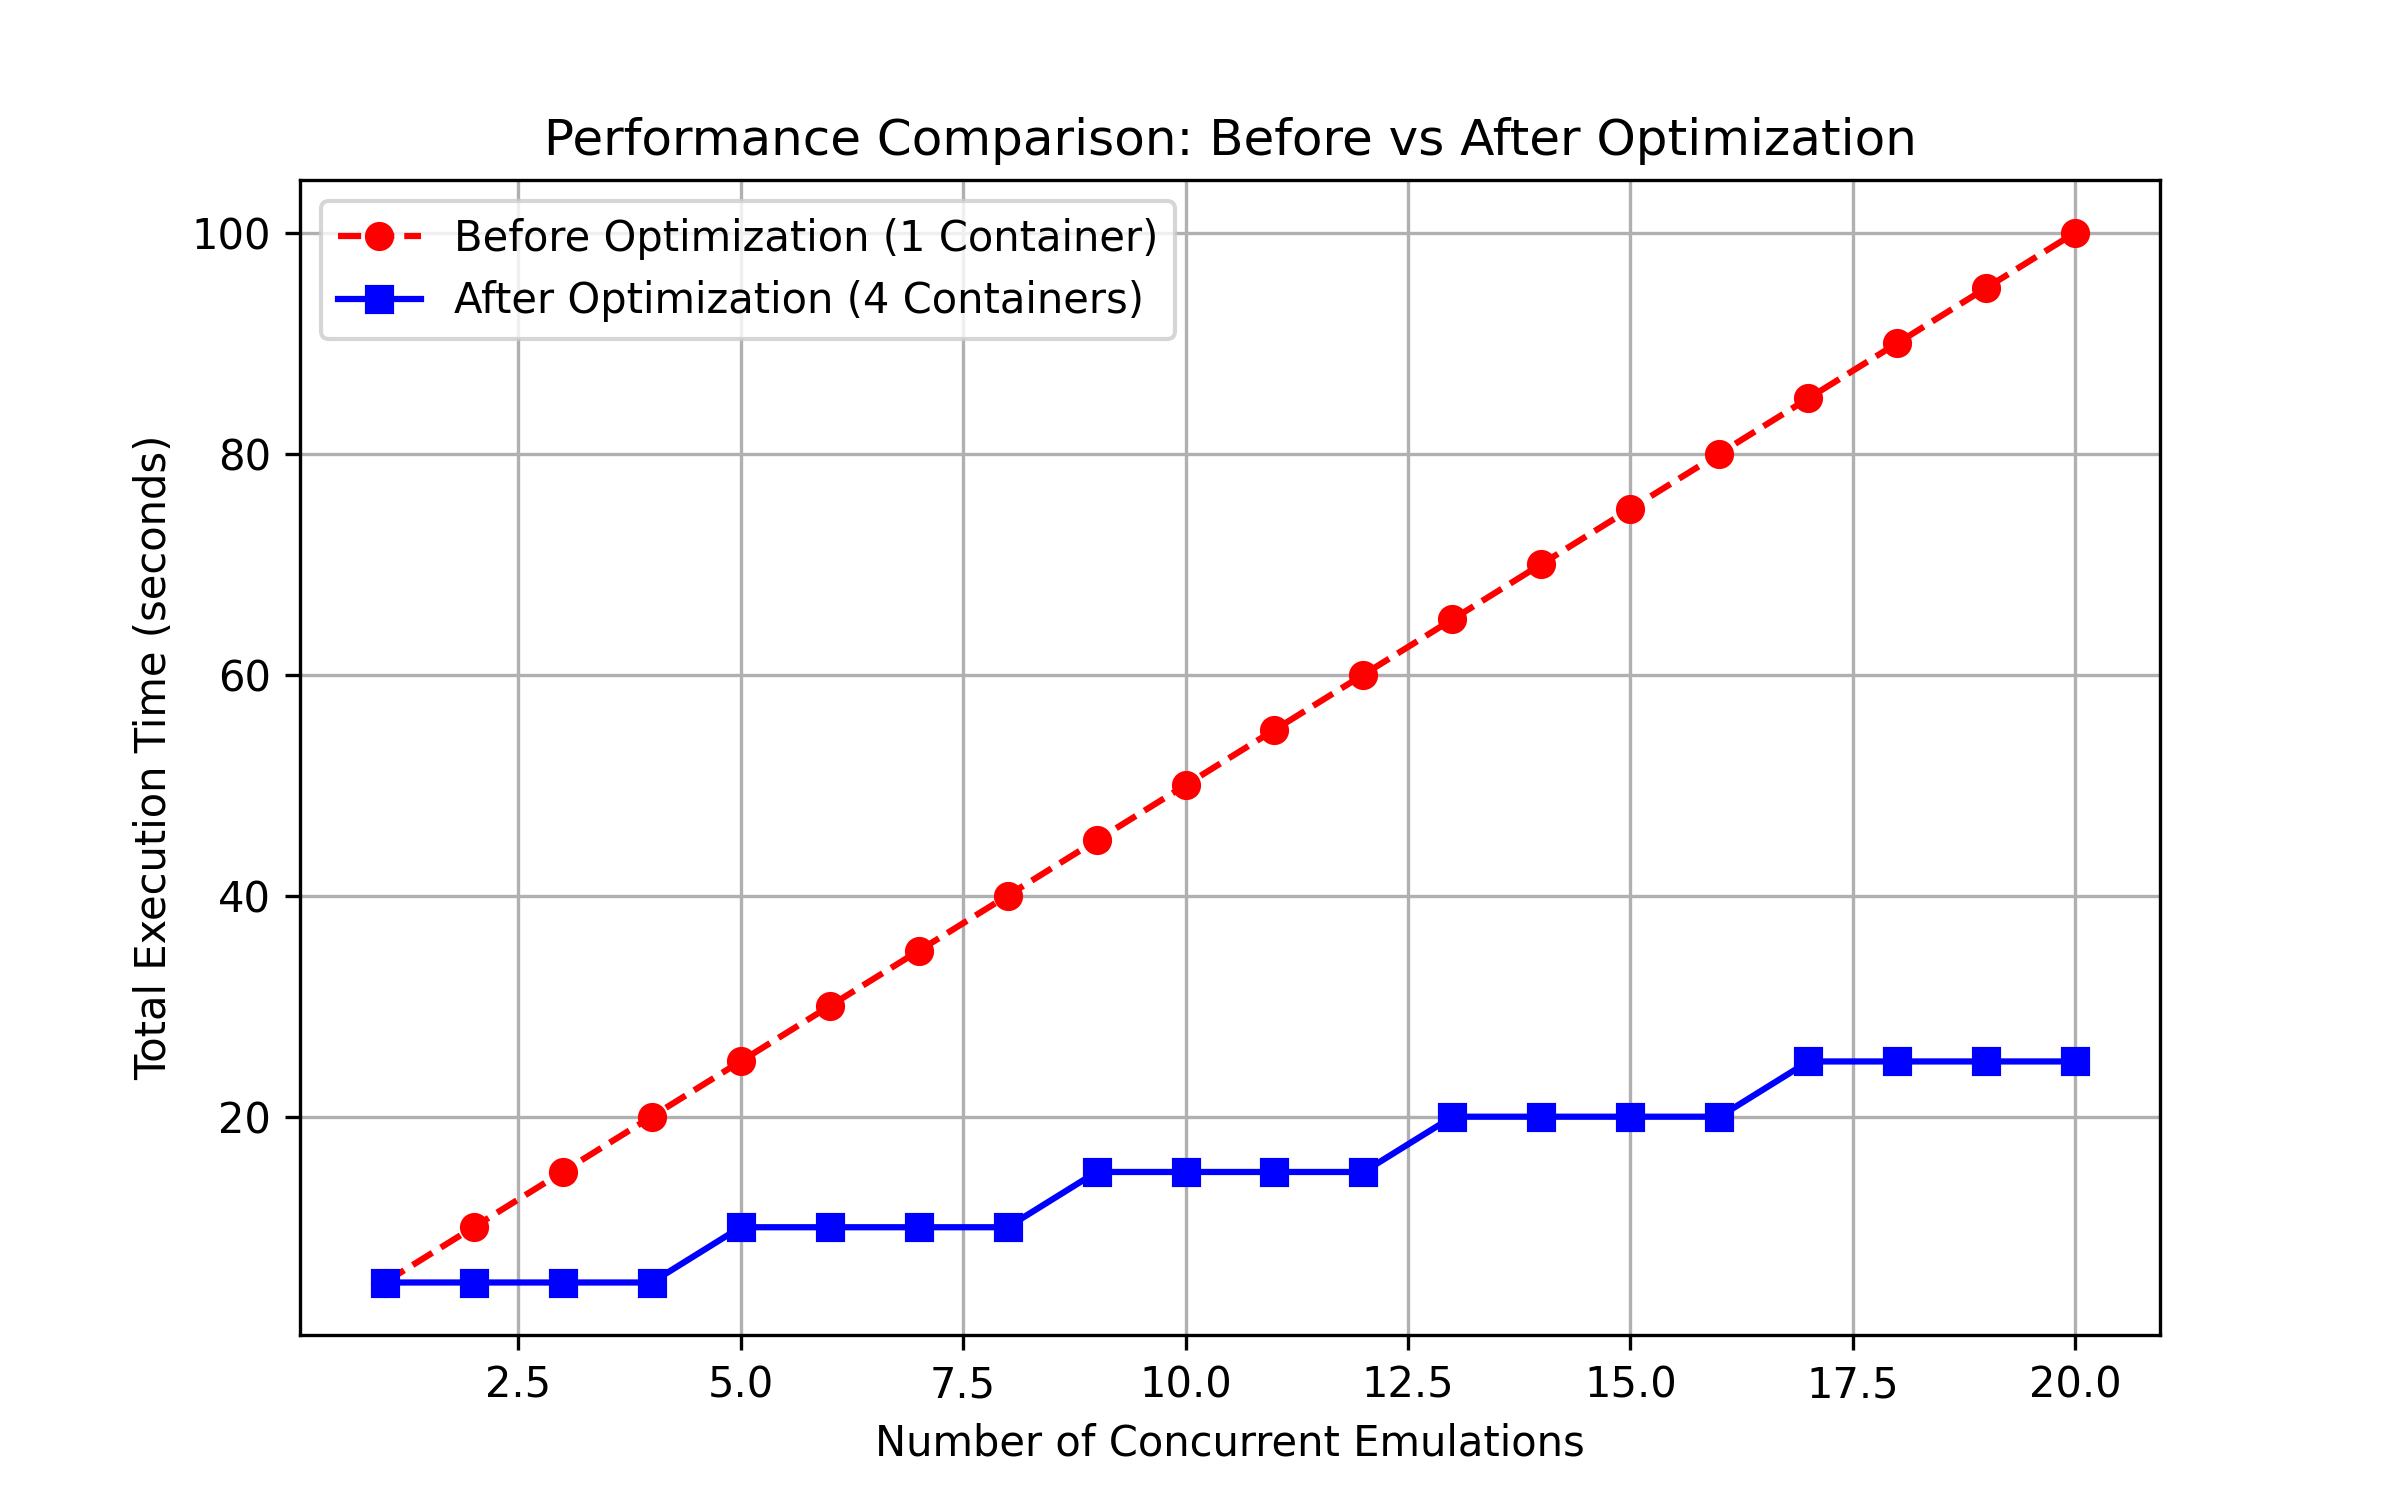
\includegraphics[width=0.8\textwidth]{performance_comparison.png}
\caption{Speedup with Increasing Container Count}
\end{figure}

\noindent\textbf{Key Benefits:}
\begin{itemize}
    \item 60\% reduction in average student wait time.
    \item Improved CPU utilization efficiency.
    \item Greater system responsiveness for simultaneous users.
\end{itemize}

% Conclusion
\section{Conclusion and Future Work}
Distributed Miminet\cite{miminet} significantly improves the practicality of teaching network courses without physical hardware. With efficient load balancing, students can now perform simulations much faster and more reliably.

\textbf{Future enhancements} include:
\begin{itemize}
    \item Kubernetes-based automatic scaling.
    \item Advanced monitoring and resource management.
    \item Fault-tolerant task execution.
\end{itemize}

The project highlights how modern virtualization and container technologies can empower education by overcoming hardware limitations.

\setmonofont{CMU Typewriter Text}
\bibliographystyle{ugost2008ls}
\bibliography{bassel_alshayeb_report}

\end{document}
